%%%
% Conférence « Comment bien démarrer son projet »
% Vendredi 13 novembre 2009
% Partie « Programmation » par Pierre-Marie de Rodat
%%%

\section{Programmation}

\subsection{Deux approches pour découper son projet}
\begin{frame}
  \begin{center}
    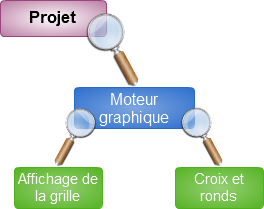
\includegraphics[scale=0.6]{images/slide1.png}
  \end{center}
\end{frame}

\begin{frame}
  \begin{center}
    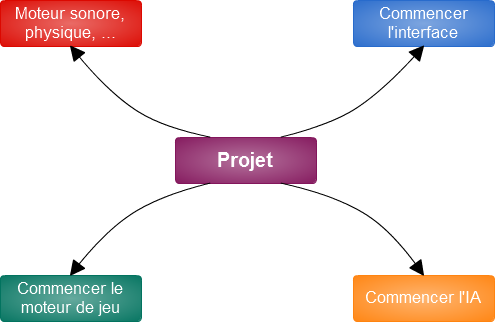
\includegraphics[scale=0.5]{images/slide2.png}
  \end{center}
\end{frame}

\begin{frame}
  \begin{block}{Un mix des deux}
    \begin{itemize}
      \item On découpe un maximum en réfléchissant avant de coder,
      \item chacun prend une partie et sait à peu près où il va,
      \item on reste dynamique.
    \end{itemize}
  \end{block}
\end{frame}